%!Mode:: "TeX:UTF-8"
\documentclass[a4paper,11pt,UTF8]{ctexart}

\usepackage{indentfirst} %缩进
\usepackage{xeCJK}    %使用系统字体
\usepackage{fancyhdr} %自定义页眉页脚
\pagestyle{empty}                   %不设置页眉页脚
\usepackage{amsmath, amsthm, amssymb, amsfonts} %数学公式
\usepackage[a4paper,left=3cm,right=3cm,top=3cm,bottom=3cm]{geometry}
%\usepackage[tmargin=1in,bmargin=1in,lmargin=1.25in,rmargin=1.25in]{geometry}.
\usepackage{booktabs} %插入表格
\usepackage[section]{placeins} %避免浮动
\usepackage{listings} %插入代码
\usepackage{ctex}     %中文宏包
\usepackage[svgnames, table]{xcolor} %彩色表格
\usepackage{algorithm}          %伪代码
\usepackage{algorithmicx}
\usepackage{algpseudocode}
\usepackage{algorithm,algpseudocode,float}
\usepackage{lipsum}
\usepackage{enumitem}           %调整列举环境
\usepackage{url}
\usepackage{fontspec,xunicode}
\defaultfontfeatures{Mapping=tex-text} %如果没有它,会有一些 tex 特殊字符无法正常使用,比如连字符。

\usepackage{graphicx}
\graphicspath{{imgs/}}

%%%%%%%%%%%%%%%%%%%%%%%%%%%%%%%%%%%%%%%%%%%%%%%%%%%%%%%%%%%%%%%%
% 缩进及行间距
%%%%%%%%%%%%%%%%%%%%%%%%%%%%%%%%%%%%%%%%%%%%%%%%%%%%%%%%%%%%%%%%
\setlength{\parindent}{22pt} %重新定义缩进长度
\setlength{\baselineskip}{20pt}  %定义行间距
%\renewcommand{\baselinestretch}{1.1} %定义行间距

%%%%%%%%%%%%%%%%%%%%%%%%%%%%%%%%%%%%%%%%%%%%%%%%%%%%%%%%%%%%%%%%
% 列表设置
%%%%%%%%%%%%%%%%%%%%%%%%%%%%%%%%%%%%%%%%%%%%%%%%%%%%%%%%%%%%%%%%
\setenumerate{fullwidth,itemindent=\parindent,listparindent=\parindent,itemsep=0ex,partopsep=0pt,parsep=0ex}
\setenumerate[2]{label=\alph*),leftmargin=1.5em}  %二级item设置
\setitemize{itemindent=38pt,leftmargin=0pt,itemsep=-0.4ex,listparindent=26pt,partopsep=0pt,parsep=0.5ex,topsep=-0.25ex}
\setdescription{itemindent=38pt,leftmargin=0pt,itemsep=-0.4ex,listparindent=26pt,partopsep=0pt,parsep=0.5ex,topsep=-0.25ex}

%%%%%%%%%%%%%%%%%%%%%%%%%%%%%%%%%%%%%%%%%%%%%%%%%%%%%%%%%%%%%%%%
% 图的标题行间距设置
%%%%%%%%%%%%%%%%%%%%%%%%%%%%%%%%%%%%%%%%%%%%%%%%%%%%%%%%%%%%%%%%
\newcommand{\bottomcaption}{%
\setlength{\abovecaptionskip}{6pt}%
\setlength{\belowcaptionskip}{6pt}%
\caption}


%%%%%%%%%%%%%%%%%%%%%%%%%%%%%%%%%%%%%%%%%%%%%%%%%%%%%%%%%%%%%%%%
% 字体定义
%%%%%%%%%%%%%%%%%%%%%%%%%%%%%%%%%%%%%%%%%%%%%%%%%%%%%%%%%%%%%%%%
\setmainfont{Times New Roman}  %默认英文字体.serif是有衬线字体sans serif无衬线字体
\setmonofont{Consolas}
\setCJKmainfont[ItalicFont={楷体}, BoldFont={黑体}]{宋体}%衬线字体 缺省中文字体为
\setCJKsansfont{黑体}
\punctstyle{hangmobanjiao}
%-----------------------xeCJK下设置中文字体------------------------------%
\setCJKfamilyfont{song}{SimSun}                             %宋体 song
\newcommand{\song}{\CJKfamily{song}}
\setCJKfamilyfont{fs}{FangSong}                      %仿宋  fs
\newcommand{\fs}{\CJKfamily{fs}}
\setCJKfamilyfont{ktgb}{KaiTi}                      %楷体2312 ktgb
\newcommand{\ktgb}{\CJKfamily{ktgb}}
\setCJKfamilyfont{yh}{Microsoft YaHei}                    %微软雅黑 yh
\newcommand{\yh}{\CJKfamily{yh}}
\setCJKfamilyfont{hei}{SimHei}                              %黑体  hei
\newcommand{\hei}{\CJKfamily{hei}}
\setCJKfamilyfont{hwxk}{STXingkai}                                %华文行楷  hwxk
\newcommand{\hwxk}{\CJKfamily{hwxk}}
%------------------------------设置字体大小------------------------%
\newcommand{\shiyanbaogao}{\fontsize{36pt}{\baselineskip}\selectfont}
\newcommand{\chuhao}{\fontsize{42pt}{\baselineskip}\selectfont}     %初号
\newcommand{\xiaochuhao}{\fontsize{36pt}{\baselineskip}\selectfont} %小初号
\newcommand{\yihao}{\fontsize{28pt}{\baselineskip}\selectfont}      %一号
\newcommand{\erhao}{\fontsize{21pt}{\baselineskip}\selectfont}      %二号
\newcommand{\xiaoerhao}{\fontsize{18pt}{\baselineskip}\selectfont}  %小二号
\newcommand{\sanhao}{\fontsize{15.75pt}{\baselineskip}\selectfont}  %三号
\newcommand{\sihao}{\fontsize{14pt}{\baselineskip}\selectfont}       %四号
\newcommand{\xiaosihao}{\fontsize{12pt}{\baselineskip}\selectfont}  %小四号
\newcommand{\wuhao}{\fontsize{10.5pt}{\baselineskip}\selectfont}    %五号
\newcommand{\xiaowuhao}{\fontsize{9pt}{\baselineskip}\selectfont}   %小五号
\newcommand{\liuhao}{\fontsize{7.875pt}{\baselineskip}\selectfont}  %六号
\newcommand{\qihao}{\fontsize{5.25pt}{\baselineskip}\selectfont}    %七号

%%%%%%%%%%%%%%%%%%%%%%%%%%%%%%%%%%%%%%%%%%%%%%%%%%%%%%%%%%%%%%%%
% 图题字体大小相同
%%%%%%%%%%%%%%%%%%%%%%%%%%%%%%%%%%%%%%%%%%%%%%%%%%%%%%%%%%%%%%%%
\usepackage{caption}
\captionsetup{font={footnotesize}}   % footnotesize = 9pt
\captionsetup[lstlisting]{font={footnotesize}}

%%%%%%%%%%%%%%%%%%%%%%%%%%%%%%%%%%%%%%%%%%%%%%%%%%%%%%%%%%%%%%%%
% 重定义枚举编号为 1),2)...
%%%%%%%%%%%%%%%%%%%%%%%%%%%%%%%%%%%%%%%%%%%%%%%%%%%%%%%%%%%%%%%%
\renewcommand{\labelenumi}{\theenumi)}

%%%%%%%%%%%%%%%%%%%%%%%%%%%%%%%%%%%%%%%%%%%%%%%%%%%%%%%%%%%%%%%%
% 标题名称中文化
%%%%%%%%%%%%%%%%%%%%%%%%%%%%%%%%%%%%%%%%%%%%%%%%%%%%%%%%%%%%%%%%
\renewcommand\figurename{\hei 图}
\renewcommand\tablename{\hei 表}
\renewcommand\lstlistingname{\hei 代码}
\renewcommand{\algorithmicrequire}{\textbf{输入:}}
\renewcommand{\algorithmicensure}{\textbf{输出:}}
\newtheorem{define}{定义}

%%%%%%%%%%%%%%%%%%%%%%%%%%%%%%%%%%%%%%%%%%%%%%%%%%%%%%%%%%%%%%%%
% 代码设置
%%%%%%%%%%%%%%%%%%%%%%%%%%%%%%%%%%%%%%%%%%%%%%%%%%%%%%%%%%%%%%%%
\lstset{
 columns=fixed,
 numbers=left,                                        % 在左侧显示行号
 numberstyle=\tiny\color{gray},                       % 设定行号格式
 frame=single,                                        % 单线背景边框
 breaklines=true,                                     % 设定LaTeX对过长的代码行进行自动换行
 keywordstyle=\color[RGB]{40,40,255},                 % 设定关键字颜色
 numberstyle=\footnotesize\color{darkgray},
 commentstyle=\it\color[RGB]{0,96,96},                % 设置代码注释的格式
 stringstyle=\rmfamily\slshape\color[RGB]{128,0,0},   % 设置字符串格式
 showstringspaces=false,                              % 不显示字符串中的空格
 language=java,                                        % 设置语言
 basicstyle=\linespread{1.0}\xiaowuhao\ttfamily,                      % 字体字号
 %lineskip=10pt,
 %baselinestretch=1,
}

%%%%%%%%%%%%%%%%%%%%%%%%%%%%%%%%%%%%%%%%%%%%%%%%%%%%%%%%%%%%%%%%
% 伪代码分页
%%%%%%%%%%%%%%%%%%%%%%%%%%%%%%%%%%%%%%%%%%%%%%%%%%%%%%%%%%%%%%%%
\makeatletter
\renewcommand{\ALG@name}{算法}
\newenvironment{breakablealgorithm}
  {% \begin{breakablealgorithm}
   \begin{center}
     \refstepcounter{algorithm}% New algorithm
     \hrule height.8pt depth0pt \kern2pt% \@fs@pre for \@fs@ruled
     \renewcommand{\caption}[2][\relax]{% Make a new \caption
       {\raggedright\textbf{\ALG@name~\thealgorithm} ##2\par}%
       \ifx\relax##1\relax % #1 is \relax
         \addcontentsline{loa}{algorithm}{\protect\numberline{\thealgorithm}##2}%
       \else % #1 is not \relax
         \addcontentsline{loa}{algorithm}{\protect\numberline{\thealgorithm}##1}%
       \fi
       \kern2pt\hrule\kern2pt
     }
  }{% \end{breakablealgorithm}
     \kern2pt\hrule\relax% \@fs@post for \@fs@ruled
   \end{center}
  }
\makeatother

% =============================================
% Part 1 Edit the info
% =============================================

\newcommand{\major}{物理学院}
\newcommand{\name}{黄阅迅,李秋阳}
\newcommand{\stuid}{PB18020631,PB18020567}
\newcommand{\group}{20}
\newcommand{\newdate}{\today}


\newcommand{\course}{电子线路实验(1)}
\newcommand{\newtitle}{差动放大器}

% =============================================
% Part 1 Main document
% =============================================
\begin{document}
\thispagestyle{empty}
\begin{figure}[h]
  \begin{minipage}{0.6\linewidth}
    \centerline{
\includegraphics[width=\linewidth]{logo.png}}
  \end{minipage}
  \hfill
  \begin{minipage}{.4\linewidth}
    \raggedleft
    \begin{tabular*}{.8\linewidth}{ll}
      学院: & \underline\major   \\
      姓名: & \underline\name    \\
      学号: & \underline\stuid   \\
      组号:  & \underline\group   \\
      日期: & \underline\newdate \\
    \end{tabular*}
  \end{minipage}
\end{figure}

\begin{table}[!htbp]
  \centering
  \begin{tabular*}{\linewidth}{llllll}
    课程名称:  \underline\course   \qquad\qquad 实验题目:  \underline\newtitle  
  \end{tabular*}
\end{table}

% =============================================
% Part 2 Main document
% =============================================

\section{实验目的}

请参看预习报告。

\section{实验原理}

请参看预习报告。

\section{实验内容与步骤}
\subsection{实验内容一}
  测量典型差动放大器的参数,并计算共模抑制比。
\subsection{实验步骤一}
\begin{figure}[htbp]
  \centering
  \fbox{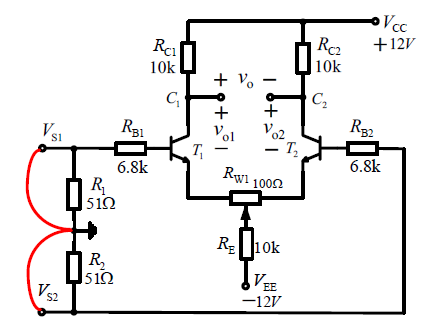
\includegraphics[width=0.5\linewidth]{nStatic.png}}
  \caption{典型差动放大器静态工作点测量示意图}
  \label{fig:nStatic}
  \end{figure}
\begin{enumerate}
  \item 按照图 \ref{fig:nStatic}连接线路,将输入信号接地,调节$R_{w1}$电位器使得$V_{C1}=V_{C2}$。用万用表直流电压
  挡位分别测量差动放大器的静态工作点参数。
  \item 将放大器输入端$V_{s2}$接地,从$V_{s1}$输入正弦信号,调节有效值为$V_{id}=20mVrms$,频率$f=1kHz$。测量差模信号的单端及双端输出信号的有效值并用示波器观察波形。
  \item 将输入端$V_{s1}$和$V_{s2}$两点连接在一起,电阻$R_1$与$R_2$从电路中断开,从$V_{s1}$和$V_{s2}$两端输入$V_{ic}=90mVrms$,频率$f=1kHz$的正弦信号。测量共模信号的单端及双端输出信号的有效值并用示波器观察波形。
  \item 根据测量数据计算单端和双端输出的共模抑制比。
\end{enumerate}
\subsection{实验内容二}
  将电阻$R_E$改为镜像恒流源,测量构成差动放大器的参数,并计算共模抑制比。
\subsection{实验步骤二}
\begin{figure}[htbp]
  \centering
  \fbox{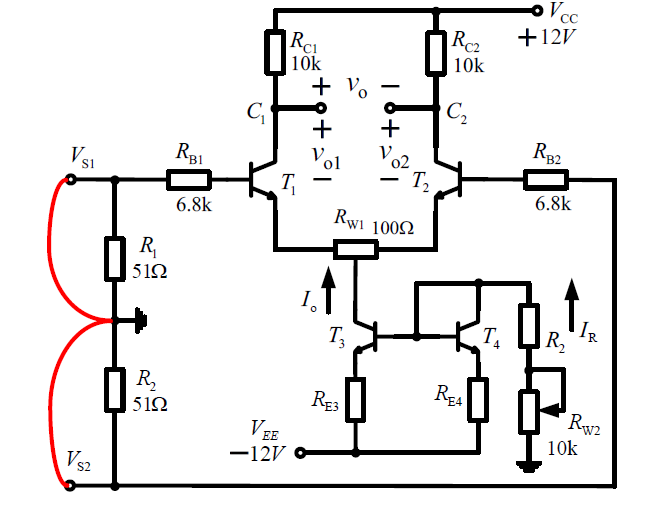
\includegraphics[width=0.5\linewidth]{sStatic.png}}
  \caption{恒流源差动放大器静态工作点测量示意图}
  \label{fig:sStatic}
  \end{figure}
\begin{enumerate}
  \item 按照图 \ref{fig:sStatic}连接线路,将输入信号接地,调节恒流源$R_{w2}=10k$电位器使得$I_0=1mA$即$V_{RC1}=5V$。用万用表直流电压
  挡位分别测量差动放大器的静态工作点参数。
  \item 将放大器输入端$V_{s2}$接地,从$V_{s1}$输入正弦信号,调节有效值为$V_{id}=20mVrms$,频率$f=1kHz$。测量差模信号的单端及双端输出信号的有效值并用示波器观察波形。
  \item 将输入端$V_{s1}$和$V_{s2}$两点连接在一起,电阻$R_1$与$R_2$从电路中断开,从$V_{s1}$和$V_{s2}$两端输入$V_{ic}=90mVrms$,频率$f=1kHz$的正弦信号。测量共模信号的单端及双端输出信号的有效值。
  \item 根据测量数据计算单端和双端输出的共模抑制比。
\end{enumerate}

\section{实验数据处理与分析}
\subsection{实验内容1}
  实验测得的静态工作点数据如表 \ref{tab:nSTab}所示。可见得到的数据都对称点的值都较为接近,比较理想。
  \begin{table}[!h!tbp]
    \caption{典型差动放大器静态工作点数据}\label{tab:nSTab}
      \centering
      \begin{tabular}{|l|c|c|c|c|c|c|}
      \hline
      数据 &$V_{C_1}$&$V_{C_2}$&$V_{E_1}$&$V_{E_2}$&$V_{B_1}$&$V_{B_2}$         \\ \hline
      值   &$6.185V$&$6.187V$&$-0.638V$&$-0.643V$&$-13.76mV$&$-15.40mV$     \\ \hline
    \end{tabular}
    \end{table}
\subsection{误差分析1}
  上述静态工作点数据,理论上对称点应完全一致,但由于实验误差,无法做到。但保证了相差小于$20mV$,从原理上可以接受,下面理论计算
  静态工作点数值。计算中采用值为$\beta=150,r_{bb'}=300\Omega,U_{BE}=0.7V$
  \begin{equation}
    \begin{aligned}
      I_{B}&=\frac{-U_{EE}-U_{BE}}{R_{B_1}+2(1+\beta)R_E+(1+\beta)\frac{R_{W_1}}{2}}=3.74\times10^{-3}mA\\
      I_{C}&=\beta I_{B}=0.561mA\\
      U_{CE}&=U_{CC}+U_{EE}-I_CR_C-2I_CR_E-I_C\frac{R_{W_1}}{2}=7.14V\\
      U_C&=U_CC-I_CR_C=6.39V\\
      U_E&=U_C-U_{CE}=-0.75V\\
      U_B&=U_E+U_{BE}=-0.05V\\
      r_{be}&=r_{bb'}+\frac{26mV}{I_B(mA)}=7.25k\Omega
    \end{aligned}
  \end{equation}
  由此可以计算出分别的相对误差(对称点取平均值)为:
  \begin{equation}
    \begin{aligned}
      \left |\frac{\Delta U_C}{U_C}\right |&=3.2\%\\
      \left |\frac{\Delta U_E}{U_E}\right |&=14\%\\
      \left |\frac{\Delta U_B}{U_B}\right |&=71\%
    \end{aligned}
  \end{equation}

  可见,除$U_C$值外,其他静态工作点值基本上只有数量级正确。这主要是因为另外两个点值基本上在$1mV$范围,因此
毫伏表的测量相当不精确造成的。但$U_C$的误差较小,说明了实验与理论基本上还是对应的。同时理论中采用了大量的近似,并且所选取
的参数值可能也与实际由偏差,因此这样的误差可以接受。实际上,对称点的电压值难以调整至一致也说明了实验的电压误差基本上是在$20mV$这个数量级的。
\subsection{实验内容2}
实验中测量得到的数据如表 \ref{tab:ndTab}所示。可见在此精度范围下,单端差模输出的有效值的绝对值基本一致。其波形图如附图1所示。可见两端的差模输出信号的反向的。
\begin{table}[!h!tbp]
  \caption{典型差动放大器差模输出数据}\label{tab:ndTab}
    \centering
    \begin{tabular}{|l|c|c|c|c|}
    \hline
    数据 &$V_{S_1}$&$V_{od_1}$&$V_{od_2}$&$V_{od}$         \\ \hline
    值   &$19.92mV$&$-808mV$&$+808mV$&$-1.610V$     \\ \hline
  \end{tabular}
  \end{table}
由此可以计算出差模信号增益为:
\begin{equation}
  \begin{aligned}
    \left |A_{ods}\right |=40.6\\
    \left |A_{od}\right |=80.8
  \end{aligned}
\end{equation}
\subsection{误差分析2}
可见实际上$v_{od}$的测量值并不完全等于$v_{od1}-V_{od2}$,但实际上这就是毫伏表读数误差造成的。
为计算理论值,画出单边小信号等效电路如图 \ref{fig:ndSmallSignal}所示。($R_b$与$R_w$未画出,认为负载$R_L\rightarrow\infty$)
\begin{figure}[htbp]
  \centering
  \fbox{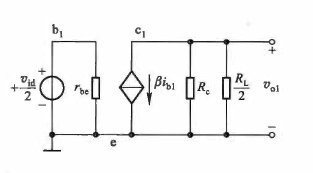
\includegraphics[width=0.5\linewidth]{ndSmallSignal.png}}
  \caption{典型差动放大器差模输出单边小信号模型}
  \label{fig:ndSmallSignal}
  \end{figure}
则可以求出输出参数为:
\begin{equation}
  \begin{aligned}
    \left | A_{vd}\right |&=\frac{\beta R_C\parallel\frac{R_L}{2}}{R_{B_1}+r_{be}+(1+\beta)\frac{R_{W_1}}{2}}=70.0\\
    \left | A_{vds}\right |&=\left |\frac{A_{vd}}{2}\right |=35.0
  \end{aligned}
\end{equation}
则可求出相对误差为:
\begin{equation}
  \begin{aligned}
    \left |\frac{\Delta A_{vd}}{A_{vd}}\right |&=15\%\\
      \left |\frac{\Delta A_{vds}}{A_{vds}}\right |&=16\%\\
  \end{aligned}
\end{equation}
首先,可见差模双端输出放大倍数并不是严格的单端输出的两倍。同时测量值与理论值偏差较大,推测是使用计算的$\beta$与$r_{bb'}$不准所导致的。
这在静态工作点时已有体现,这个误差经过放大变得更加大。同时使用的元件也有一定的误差,小信号分析本身也具有一定误差,并未考虑频率响应。
\subsection{实验内容3}
实验测得的共模输出数据如表 \ref{tab:ncTab}所示。可见共模输出电压较小。

\begin{table}[!h!tbp]
  \caption{典型差动放大器共模输出数据}\label{tab:ncTab}
    \centering
    \begin{tabular}{|l|c|c|c|c|}
    \hline
    数据 &$U_{i}$&$U_{oc_1}$&$U_{oc_2}$&$U_{oc}$         \\ \hline
    值   &$90.1mV$&$-43.9mV$&$-46.8mV$&$1.610mV$     \\ \hline
  \end{tabular}
  \end{table}
则可以计算出共模电压增益为(单端输出时取平均值):
\begin{equation}
  \begin{aligned}
    \left | A_{ucs}\right |&=0.503\\
    \left | A_{ucs}\right |&=0.0306
  \end{aligned}
\end{equation}
结合上一实验内容,可以算出差模抑制比为:
\begin{equation}
  \begin{aligned}
    K_{CMRs}&=80.7\\
    K_{CMR}&=2.64\times10^{3}
  \end{aligned}
\end{equation}
\subsection{误差分析3}
同样有,单端输出和双端输出电压值并不完全匹配的问题。
单端输出时半边小信号模型如图\ref{fig:ncSmallSignal}所示。($R_b$与$R_w$未画出,认为负载$R_L\rightarrow\infty$)
\begin{figure}[htbp]
  \centering
  \fbox{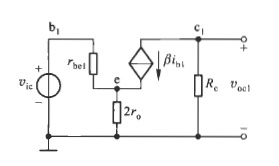
\includegraphics[width=0.5\linewidth]{ncSmallSignal.png}}
  \caption{典型差动放大器共模输出单边小信号模型}
  \label{fig:ncSmallSignal}
  \end{figure}
则可以求出共模输出参数以及结合上一内容模型可以算出差模抑制比为
\begin{equation}
  \begin{aligned}
    \left | A_{vcs}\right |&\approx\frac{R_c\parallel R_L}{2R_E}=0.500\\
    \left | A_{vc}\right |&=0.00\\
    K_{CMRs}&=\left |\frac{A_{vds}}{A_{vcs}}\right |=70.0\\
    K_{CMR}&=\infty
  \end{aligned}
\end{equation}
可见,双端输出时的抑制比并不可能做到理想的正无穷程度,共模输出增益也不可能是0,但前者也非常大,后者也相当小,比较符合理论预测。
其他量的相对误差为:
\begin{equation}
  \begin{aligned}
      \left |\frac{\Delta A_{cds}}{A_{cds}}\right |&=0.6\%\\
      \left |\frac{\Delta K_{CMRs}}{K_{CMRs}}\right |&=15\%
  \end{aligned}
\end{equation}
可见,共模单端输出的相对误差意外得小,这是因为其计算时几乎没有用到三极管的预设参数。侧面证明,计算误差来源可能主要是三极管的参数不准。
单端共模抑制比的误差仍较大,原因如前所述。


\section{实验总结}
blablabla
\section{实验思考题}
balabalabala

\begin{appendix}

\section{代码示例}

\begin{lstlisting}[caption={一段C代码},captionpos=b]
#include <stdio.h>
int main (int argc, char *argv[]){
  printf("Hello world!");
}
\end{lstlisting}

\section{表格示例}
表 \ref{tab:tab1}与表 \ref{tab:tab2}展示了表格示例
\begin{table}[!h!tbp]
\caption{一个简单的表格}\label{tab:tab1}
  \centering
  \begin{tabular}{|l|c|c|}
	\hline
	功能          &WEB         &APP         \\ \hline
	注册          &$\surd$     &$\surd$     \\ \hline
	登录          &$\surd$     &$\surd$     \\ \hline
	推送          &$\times$    &$\surd$     \\ \hline
\end{tabular}
\end{table}

\begin{table}[!h!tbp]
\caption{自定义表格}\label{tab:tab2}
  \centering
\begin{tabular*}{0.75\textwidth}{@{\extracolsep{\fill}}lcc}
    \toprule
    功能          &WEB         &APP         \\
    \midrule
    注册          &$\surd$     &$\surd$     \\
    登录          &$\surd$     &$\surd$     \\
    推送          &$\times$    &$\surd$     \\
    \bottomrule
\end{tabular*}
\end{table}


\section{图片示例}
图 \ref{fig:logo}展示了一个图片示例。
\begin{figure}[htbp]
\centering
\fbox{
\includegraphics[width=0.5\linewidth]{logo}}
\caption{blablabla}
\label{fig:logo}
\end{figure}

\section{公式示例}
式 (\ref{eqa:01})展示了一个公式的例子。
\begin{equation}
S_n = \frac{X_1 + X_2 + \cdots + X_n}{n}
      = \frac{1}{n}\sum_{i}^{n} X_i
\label{eqa:01}
\end{equation}




\end{appendix}

\end{document}
